\documentclass[11pt]{article}
\usepackage{scribe}
\usepackage{graphicx}

% Uncomment the appropriate line
%\Scribe{Your name}

\Scribes{Frendy Lio Can}
\LectureDate{September 23, 2020}
\LectureTitle{Homework Assignment \#1}

%\usepackage[mathcal]{euscript}


\begin{document}

\MakeScribeTop

%\paragraph{This is a paragraph heading} Paragraph.

%%%%%%%%%%%%%%%%%%%%%%%%%%%%%%%%
% PROBLEM 1
%%%%%%%%%%%%%%%%%%%%%%%%%%%%%%%%
\paragraph{\noindent\textbf{\LARGE{Problem 1}}}

% Start of Explaining

\begin{flushleft}
a) \\
If the input were a Dirac impulse at $x_i = x_1 \Rightarrow x_o = Mx_1 \quad \therefore{}$
\end{flushleft}   
\begin{equation*}
\begin{split}
    \delta(x - x_i) \xrightarrow{S} h(x ; x_i) & = \delta(x - x_o) = \delta (x - M x_1) = \delta(x - M x_i) \\
    \therefore{}\\
    h(x; x') & = \delta(x - Mx')
\end{split}
\end{equation*}

\begin{flushleft}
b) 
\end{flushleft}   
\begin{equation*}
\begin{split}
    g(x)    = & \int_{-\infty}^{\infty} f(x')h(x;x')dx' \\
            = & \int_{-\infty}^{\infty} f(x')\delta(x -Mx')dx'\\
            = & \int_{-\infty}^{\infty} f(x')\delta(Mx' - x )dx' \quad \text{, symmetry property.} \\
            = & \int_{-\infty}^{\infty} f(x')\delta[M(x' - \frac{x}{M})] dx'\\
            = & \frac{1}{|M|} f(\frac{x}{M}) \quad \text{, using scaling and sifting property of Dirac function.} 
\end{split}
\end{equation*}

\begin{flushleft}
c) \\
From the notes, section 1.4.2. A 1D pinhole models illustrate a magnification or mirroring system; this implies that is a shift-variant system.
This is because the PSF does not depend solely on the difference between input and output coordinates.
\newline \newline
Proof: 
\newline \newline
For $g_1:$
\end{flushleft}   
\begin{equation*}
\begin{split}
    g_1(x)          = &f(x) \xrightarrow{S} g(x) \rightarrow shift(x_0)\\
    g_{1_a}(x)      = &f(x) \xrightarrow{S} g(x) = \frac{1}{|M|} f(\frac{x}{M}) \\
    g_1(x)          = &g_{1_a}(x)  \rightarrow shift(x_0)  = \frac{1}{|M|} f(\frac{x}{M} - x_0) \\
    \therefore{} & \\
    g_1(x) = & \frac{1}{|M|} f(\frac{x}{M} - x_0)  
\end{split}
\end{equation*}
\begin{flushleft}
For $g_2:$
\end{flushleft} 
\begin{equation*}
\begin{split}
    g_2(x)          = &f(x) \rightarrow shift(x_0) \xrightarrow{S} g(x)\\
    g_{2_a}(x)      = & f(x) \rightarrow shift(x_0)    =  f(x - x_0) \\
    g_2(x)          = & g_{2_a}(x)   \xrightarrow{S} g(x) =  \frac{1}{|M|} f(\frac{x - x_0}{M}) \\
    \therefore{} & \\
    g_2(x) = & \frac{1}{|M|} f(\frac{x - x_0}{M})  
\end{split}
\end{equation*}
\begin{flushleft}
Therefore, we can conclude it is shift-variant because $g_1 \neq g_2$.
\end{flushleft} 

%%%%%%%%%%%%%%%%%%%%%%%%%%%%%%%%
% PROBLEM 2
%%%%%%%%%%%%%%%%%%%%%%%%%%%%%%%%
\paragraph{\noindent\textbf{\LARGE{Problem 2}}}

\begin{flushleft}
a) \newline
If $g(t) \xleftrightarrow{CTFT} G(f) \Rightarrow g(t-a) \xleftrightarrow{CTFT} e^{-i2\pi af}G(f)$:
\newline\newline
Proof:
\newline
We know that
\end{flushleft} 
\begin{equation*}
\begin{split}
G(f) = & \int_{-\infty}^{\infty} g(t)e^{-i2\pi ft} dt
\end{split}
\end{equation*}
\begin{flushleft}
Let $z(t) = g(t - a )$ and $\tau = t - a \rightarrow d\tau = dt$; thus,
\end{flushleft} 
\begin{equation*}
\begin{split}
    z(t)  & \xrightarrow{CTFT} Z(f) \\
    Z(f)  & = \int_{-\infty}^{\infty} g(t - a )e^{-i2\pi ft} dt = \\ 
                            & = \int_{-\infty}^{\infty} g(\tau )e^{-i2\pi f(\tau + a)} d\tau \\ 
                            & = \int_{-\infty}^{\infty} g(\tau )e^{-i2\pi f\tau} e^{-i2\pi fa} d\tau \\ 
                            & = e^{-i2\pi fa} \int_{-\infty}^{\infty} g(\tau )e^{-i2\pi f\tau} d\tau \\ 
                            & = e^{-i2\pi fa} G(f) \\
                            & = e^{-i2\pi fa} G(f) \\
                            \therefore{}
\end{split}
\end{equation*}
\begin{equation*}
\begin{split}
    z(t) \xleftrightarrow{CTFT} e^{-i2\pi fa} G(f) \Rightarrow g(t - a) \xleftrightarrow{CTFT} e^{-i2\pi fa} G(f)
\end{split}
\end{equation*}

\begin{flushleft}
b) \newline
If $g(x,y) \xleftrightarrow{CSFT} G(u,v) \Rightarrow g(\frac{x}{a}, \frac{y}{b}) \xleftrightarrow{CSFT} |ab|G(au, bv)$:
\newline\newline
Proof:
\newline
We know that
\end{flushleft} 
\begin{equation*}
\begin{split}
G(u,v) = & \int_{-\infty}^{\infty} \int_{-\infty}^{\infty} g(x,y)e^{-i2\pi (ux + vy)} dxdy
\end{split}
\end{equation*}
\begin{flushleft}
Let $z(x, y) = g(\frac{x}{a}, \frac{y}{b} )$ and 
    $\alpha = \frac{x}{a} \rightarrow d\alpha = \frac{1}{a} dx$; 
    $\beta = \frac{y}{b} \rightarrow d\beta = \frac{1}{b} dy$
thus,
\end{flushleft} 
\begin{equation*}
\begin{split}
    z(x,y)  & \xrightarrow{CSFT} Z(u,v) \\
    Z(u,v)  & = \int_{-\infty}^{\infty} \int_{-\infty}^{\infty} g(\frac{x}{a},\frac{y}{b})e^{-i2\pi (ux + vy)} dxdy = \\ 
            & = \int_{-\infty}^{\infty} \int_{-\infty}^{\infty} g(\alpha,\beta)e^{-i2\pi (au\alpha + bv\beta)} ad\alpha \cdot bd\beta  \\
            & = |ab|\int_{-\infty}^{\infty} \int_{-\infty}^{\infty} g(\alpha,\beta)e^{-i2\pi (au\alpha + bv\beta)} d\alpha \cdot d\beta  \\    
            & = |ab| \cdot G(au, bv) \\
\end{split}
\end{equation*}
\begin{flushleft}
Note that if $ab < 0, \quad da\alpha \cdot db\beta < 0 $, will flip the integrals to $-\infty$ to $\infty$.
\end{flushleft} 
\begin{equation*}
\begin{split}
    Z(u,v) & = |ab| \cdot G(au, bv) \\
            \therefore{}
\end{split}
\end{equation*}
\begin{equation*}
\begin{split}
    z(x,y) \xleftrightarrow{CSFT} |ab| \cdot G(au, bv) \Rightarrow g(\frac{x}{a}, \frac{y}{b} ) \xleftrightarrow{CSFT} |ab| \cdot G(au, bv)
\end{split}
\end{equation*}

\begin{flushleft}
c) \newline
If $g(\begin{bmatrix}
    x \\ y
\end{bmatrix}) \xleftrightarrow{CSFT} 
G(\begin{bmatrix}
    u \\ v
\end{bmatrix}) \Rightarrow g(A\begin{bmatrix}
    x \\ y
\end{bmatrix}) \xleftrightarrow{CSFT} 
|det(A)|^{-1}G((A^{-1})^T\begin{bmatrix}
    u \\ v
\end{bmatrix})$
\newline\newline\newline
Proof:
\newline
We know that
\end{flushleft} 
\begin{equation*}
\begin{split}
G(\begin{bmatrix}
    u \\ v
\end{bmatrix}) =  & \int_{-\infty}^{\infty} \int_{-\infty}^{\infty} 
g(\begin{bmatrix}
    x \\ y
\end{bmatrix})
e^{-i2\pi 
    \begin{bmatrix}
        x & y
    \end{bmatrix}    
    \begin{bmatrix}
        u \\ v
    \end{bmatrix}
}
dxdy
\end{split}
\end{equation*}
\begin{flushleft}
Let $z(x, y) =
g(A\begin{bmatrix}
    x \\ y
\end{bmatrix})$ and 
    $\omega = A\begin{bmatrix}
        x \\ y
    \end{bmatrix} \rightarrow d\omega = |det(A)|dx dy$
thus,
\end{flushleft} 
\begin{equation*}
\begin{split}
    \omega &= A \begin{bmatrix}
        x \\ y
    \end{bmatrix} \Leftrightarrow\\
    \Leftrightarrow &A^{-1} \omega = A^{-1}A\begin{bmatrix}
        x \\ y
    \end{bmatrix} \\
    \Leftrightarrow & A^{-1} \omega = \begin{bmatrix}
        x \\ y
    \end{bmatrix} \\
    \Leftrightarrow & (A^{-1} \omega)^T = (\begin{bmatrix}
        x \\ y
    \end{bmatrix})^T \\
    \Leftrightarrow  & \omega^T(A^{-1})^T =\begin{bmatrix}
        x & y
    \end{bmatrix}
\end{split}
\end{equation*}
\begin{equation*}
\begin{split}
    z(x,y)  & \xrightarrow{CSFT} Z(u,v) \\
    Z(u,v)  & = \int_{-\infty}^{\infty} \int_{-\infty}^{\infty} 
    g(A\begin{bmatrix}
        x \\ y
    \end{bmatrix})e^{-i2\pi 
    \begin{bmatrix}
        x & y
    \end{bmatrix}    
    \begin{bmatrix}
        u \\ v
    \end{bmatrix}
}dx dy \\ 
& = \int_{-\infty}^{\infty} \int_{-\infty}^{\infty} 
g(\omega)e^{-i2\pi \omega^T(A^{-1})^T 
\begin{bmatrix}
    u \\ v
\end{bmatrix}
} |det(A)|^{-1} d\omega \\
& = |det(A)|^{-1}\int_{-\infty}^{\infty} \int_{-\infty}^{\infty} 
g(\omega)e^{-i2\pi \omega^T(A^{-1})^T 
\begin{bmatrix}
    u \\ v
\end{bmatrix}
}  d\omega \\
& = |det(A)|^{-1}G((A^{-1})^T\begin{bmatrix}
    u \\ v
\end{bmatrix}) 
\\ \therefore{}
\end{split}
\end{equation*}
\begin{equation*}
\begin{split}
    z(x,y) \xleftrightarrow{CSFT} 
    |det(A)|^{-1}G((A^{-1})^T\begin{bmatrix}
        u \\ v
    \end{bmatrix})
\Rightarrow g(A\begin{bmatrix}
    x \\ y
\end{bmatrix})
 \xleftrightarrow{CSFT} 
 |det(A)|^{-1}G((A^{-1})^T\begin{bmatrix}
    u \\ v
\end{bmatrix})
\end{split}
\end{equation*}
%%%%%%%%%%%%%%%%%%%%%%%%%%%%%%%%
% PROBLEM 3
%%%%%%%%%%%%%%%%%%%%%%%%%%%%%%%%
\paragraph{\noindent\textbf{\LARGE{Problem 3}}}

\begin{flushleft}
a) \newline
$H(\rho) = |\rho| \quad \because$ 
\end{flushleft}
\begin{equation*}
\begin{split}
    g_\theta (r) &= \int_{-\infty}^{\infty} |\rho| P_\theta (\rho)e^{i2\pi \rho r} d\rho = \\
                & = CTFT^{-1} {|\rho|P_\theta (\rho)} \\
                & = h(r) * P_\theta(r) \\
    G_\theta(\rho) & = |\rho|P_\theta(\rho) \\
    & = H(\rho)P_\theta(\rho) \\
    |\rho|P_\theta(\rho) & = H(\rho)P_\theta(\rho) \Rightarrow H(\rho) = |\rho|\\
\end{split}  
\end{equation*}
\begin{flushleft}
b) \newline
No, it is not practical. This is because $|\rho|$ is a ramp function; this means that it will take any frequencies as input which create noise.
Thus, if we have more noise, it will create more inaccurate output.
\end{flushleft}
\begin{flushleft}
c) \newline

The new function is more practical than $H(\rho)$. This is because the rect function will filter the noises for high frequency.
\newline

A limitation of this new function is that it might filter for high frequencies.

\begin{figure}[htbp]
    \centerline{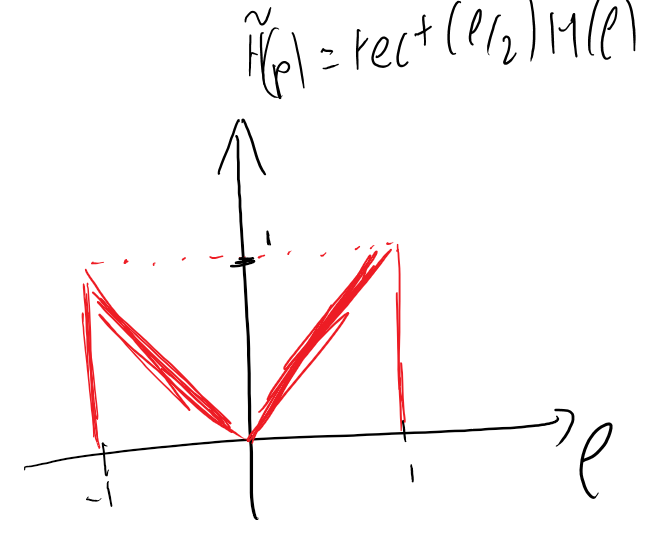
\includegraphics[scale=.5]{Capture.PNG}}
    \caption{Sketch}
    \label{fig}
\end{figure}

\end{flushleft}
\end{document}
